\section{Theoretical Guarantees}~\label{sec:guarantee}
In this section, we first prove the soundness of \tool\ and then discuss the detection capability as compared to existing approaches.
Both the proof and discussion are in the context of sequential consistency model~\cite{scmodel}.

\begin{mytheorem}[Soundness]
The trace $\tau'$ computed by the solver is a feasible trace for the concurrent program.
\end{mytheorem}

\begin{proof}\let\qed\relax
The proof consists of two parts: (1) the trace is feasible, and (2) the trace can be generated by the program. We sketch the proof as follows.
\begin{itemize}
\item  $\tau'$ is feasible. Researchers~\cite{chao,maximal} point out a 
trace is feasible iff it satisfies the sequential consistency, 
i.e., $\forall object\ o, \tau'\downarrow_{o}$ satisfies the serial 
specification of the object $o$. If  all the events considered are of 
the types in Table~\ref{Ta:syntax}, then the sequential consistency 
precisely means the following: (1) read-write consistency, i.e., each 
read event of a variable should contain the value written by the most 
recent write event, and (2) the synchronization consistency, e.g., the 
acquisition and release of a lock should not interleave with other 
lock operations of the same lock, the start event of a thread should 
follow the fork event of the parent thread. Our inter-thread data 
flow constraints guarantee the read-write consistency among shared 
locations. The SSA form encodes the read-write consistency among local 
variables. The synchronization consistency is also captured as constraints 
in our solver. 
\item $\tau'$ can be generated by the program, i.e., for each 
thread $t$, $\tau'\downarrow_{t}$ can be generated by the corresponding 
thread code. This claim requires that,  for any two adjacent 
events $e$ and $e'$ in  $\tau'\downarrow_{t}$, (1) if $e$ is not a 
branch, $inst^e$ and $inst^{e'}$ should be adjacent in the code; (2) 
if $e$ is a branch, $inst^e$ and $inst^{e'}$ should be adjacent in terms
of control flow and the $inst^e$ should be evaluated as the boolean 
value implied by $inst^{e'}$. We derive the trace  through either 
concrete execution or precise modeling of unexplored branches, 
which satisfies the requirements and guarantees the correctness of the claim.
\end{itemize}
\end{proof}



\begin{mydiscussion}[Detection Capability]
Our technique has stronger detection capability than existing techniques~\cite{yannis,pldi14,Said:2011}.
\end{mydiscussion}

First, to the best of our knowledge, none of the existing techniques 
automatically explore the un-executed branches by relaxing the schedules, whereas \tool enables this.
Second, assume we disable the exploration of un-executed branches and all 
techniques start with the same trace. Our technique still explores more 
traces. Figure~\ref{fig:discuss} illustrates the difference, where two 
vertical lines represent the progress of two threads and the circles 
with numbers denote events with ids. 
Existing techniques require the reads to read the same values, and hence
enforce the schedule order $e_5 \rightarrow e_6$ and $e_2\rightarrow e_3$. 
We allow the reads to read different values from different writes as long as 
the feasibility is preserved. Comparatively, we enforce a weaker 
schedule order  $e_4 \rightarrow e_6$ and $e_2\rightarrow e_3$, which 
allows more scheduling, e.g., the concurrent execution of $e_7$ (or 
some event after $e_7$) and $e_5$.

However, \tool has not reached the maximum bound of sound exploration.
% does not identify the maximal set of traces 
%from a single trace. 
The underlying reason is that, we still enforce the schedule for 
preserving the base object, e.g., $e_2\rightarrow e_3$. It is possible 
to further relax the schedule so that $e_3$ reads from $e_1$, but 
this requires challenging reasoning of the field accesses as their base 
objects become uncertain. We plan to explore this idea in future work.




\begin{figure}[htp]
\centering
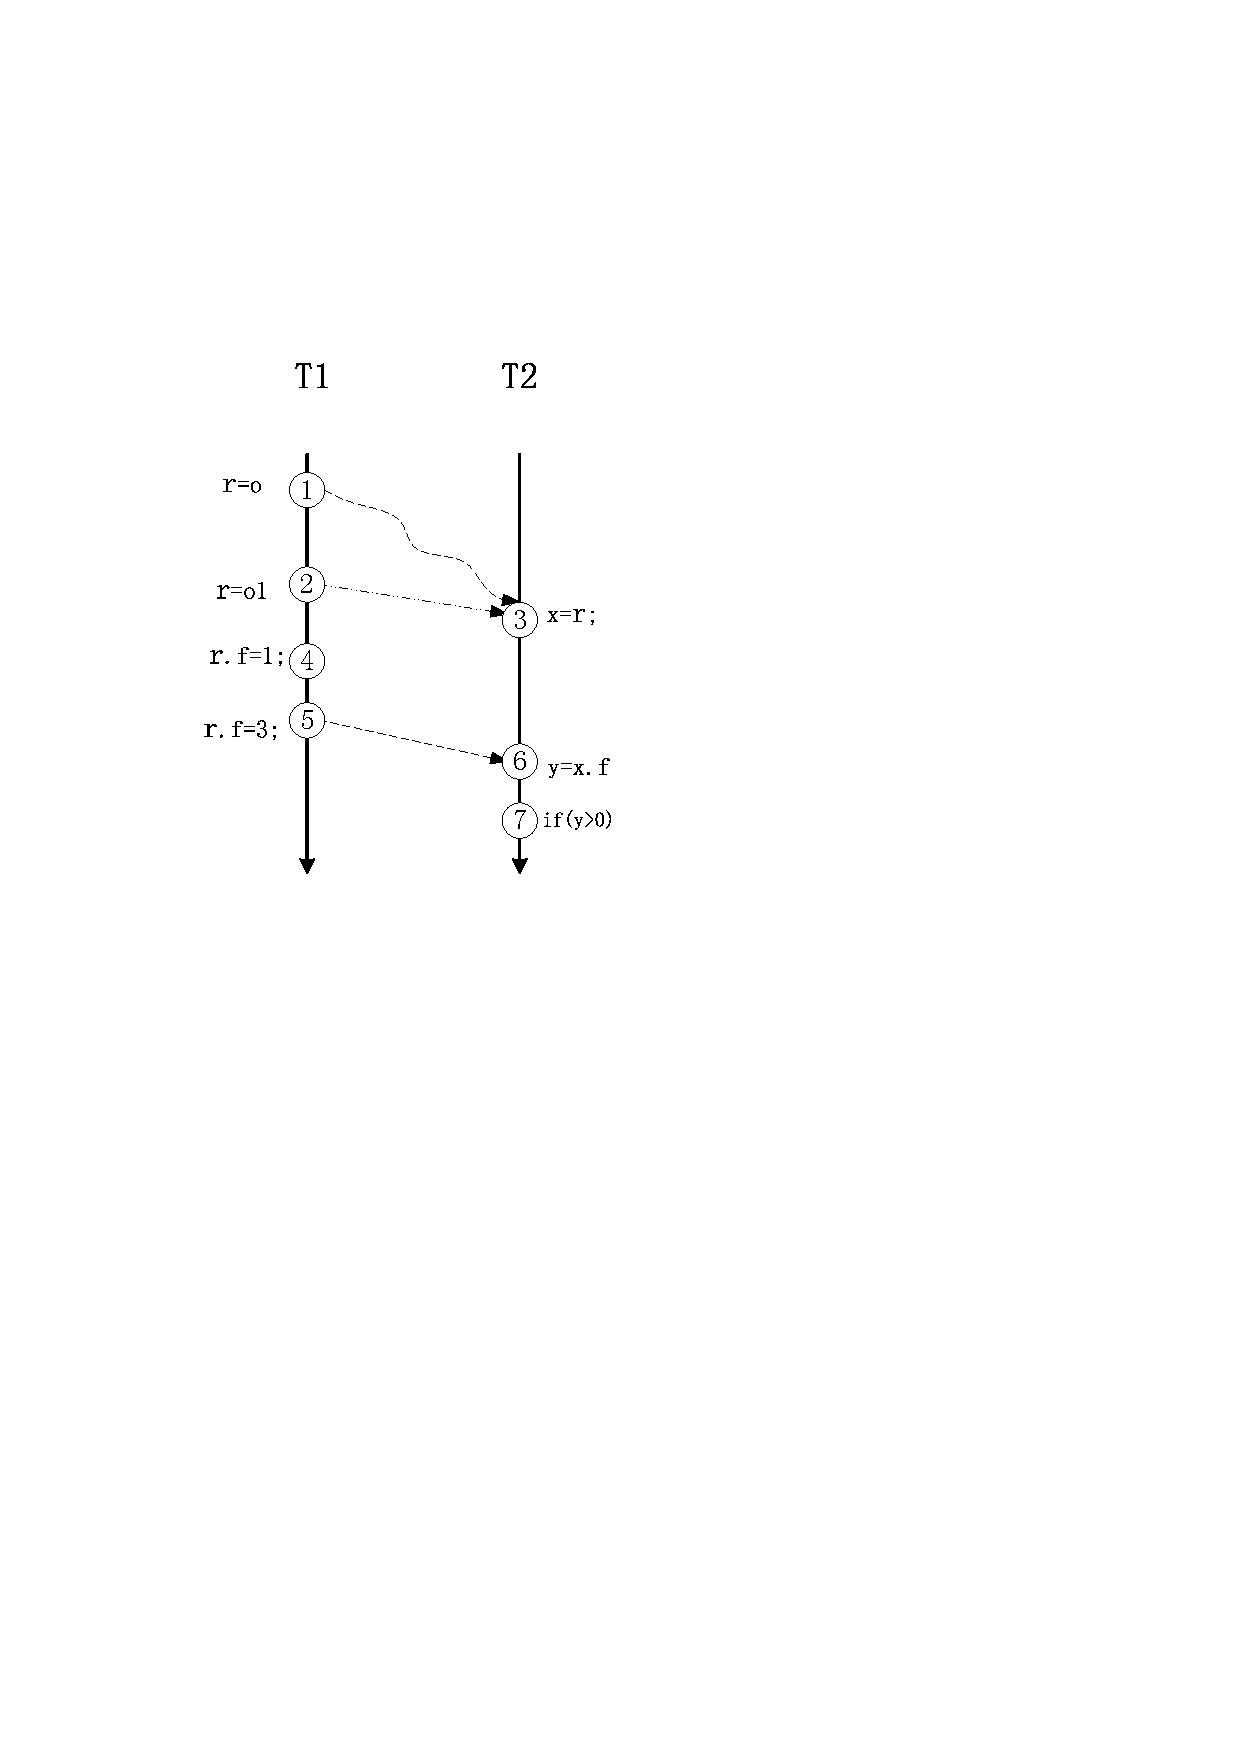
\includegraphics[width=4cm,height=4cm]{figs/Visio-discuss.pdf}
\caption{Illustration of Detection Capability.}\label{fig:discuss}
\end{figure}




%
%In this section, we prove formally the soundness of \tool.
%
%Researchers~\cite{pldi14,maximal} propose two axioms, {\em prefix closedness} and {\em local determinism}, which we adapt to establish our feasibility guarantee. 
%Suppose $\mathcal{F}$ denotes the domain of feasible traces.
%
%
%Intuitively, Prefix closedness means that if a trace is feasible, then the trace is still feasible after we discard the events after a point. The underlying reason is that the events after a point cannot affect the events before it. More formally,
%
%\begin{myaxiom}[Prefix closedness]~\label{axiom:prefix}
%If $t_1$ $t_2$ $\in \mathcal{F}$, then $t_1 \in \mathcal{F}$. 
%\end{myaxiom}
%
%
%
%
%Intuitively, local determinism says that only the previous events of the same thread determine the existence of an event. For example, the existence of an event is only determined by the branch  thread-locally. However, the value read by an event may be affected by another thread because a shared read reads from the most recent write, which may come from a different thread. The value in other events, such as branch or write,  are locally determined too.
%More formally,
%
%
%
%
%
%\begin{myaxiom}[Local determinism]~\label{axiom:local}
%Assume $t_1e_1, t_2 \in \mathcal{F}$, and $t_1|thread(e_1)\approx t_2|thread(e_1)$, where $\approx$ denotes the two traces are equal if the data values in the read and write events are ignored, 
%Each event is determined by the previous events in the same thread. There are four cases:
%\begin{itemize}
%%TODO refine it.
%\item {\bf Branch\ }. If op($e_1$)=branch, and $e_1$ is in the form of $x<y$ (without loss of generality), then there exists values $v_x$, $v_y$ such that $t_2 e_1 [v_x/data_x, v_y/data_y] \in \mathcal{F}$. Here $e_1 [v_x/data_x]$ represents that we replace the value of $x$ from $data_x$ to $v_x$ in $e_1$.
%\item {\bf Read\ }. If op($e_1$)=read, and $e_2$ is a read event that is identical to $e_1$ except that it may read a different value, and $t_2 e_2$ is consistent, then $t_2 e_2 \in \mathcal{F}$.
%\item {\bf Write\ }. If op($e_1$)=write, and there is a value $v$ such that $t_2 e_1[v/data]\in \mathcal{F}$. 
%\item {\bf Others \ }. If op($e_1$) is of type different from above and $t_2 e_1$ is consistent, then $t_2 e_1 \in \mathcal{F}$.
%\end{itemize}
%
%Here, the consistency is defined as follows. 
%A trace is consistency iff it satisfies 
%\end{myaxiom}
%
%The local determinism resembles the version in ~\cite{pldi14,maximal}. A crucial difference is that, for the branch event, we do not require all reads thread locally before it to read the identical values as in the original trace $t_1 e_1$. Instead, we allow the previous reads to read different values as long as the branch event is evaluated to the same boolean value, which guarantees the existence of the following events. Such relaxation allows us to find more races, while still preserving the feasibility. 
%
%
%An important assumption of ours is, we assume all local accesses are recorded in the trace so that we can determine the boolean status of a branch event computationally. ~\cite{pldi14}, which assume the local accesses are not recorded and cannot determine the status computationally, have to enforce the reads before a branch to read the same values, leading to a weaker feasibility criterion. We believe our axiom captures the real-world scenario more faithfully.
%Another important assumption is for the read-write consistency, i.e., we assume the heap invariant, so that we know exactly which reads correspond to which writes in the predicted run.
%
%%\begin{myaxiom}
%%A set of traces $\mathcal{F}$ is feasible if it satisfies prefix closedness and local determinism axioms. 
%%\end{myaxiom}
%
%
%
%They are called axioms because they are the rules that the sequentially consistent system~\cite{maximal} should follow.
%We refer the readers to the detailed discussion~\cite{maximal, pldi14}.
%
%
%
%%TODO what is \Phi
%\begin{mytheorem}[Soundness]
%All traces in the closure $closure(t, \Phi)$, which includes $t$ and is closed under the derivations in Axioms~\ref{axiom:prefix}~\ref{axiom:local}, are feasible.
%\end{mytheorem}
%
%%$\theta_1(expr(e_1))=\theta_2(expr_{e_1})$, then $t_2 \e_1 \in \mathcal{F}$. Here $\theta_1, \theta_2$ represent the mappings between variables and values established prior to $e_1$ by the same thread $thread(e_1)$. $expr(e_1)$ is a helper function that returns the expression in the branch condition. 
%\begin{proof}
%We order the traces in $closure(t)$ as, $t_0=t, t_1, t_2, t_3, \dots t_n$. Clearly, $t_0$ is feasible. In the following, we prove by induction, i.e., assume $t_{n}$ is feasible, then $t_{n+1}$ which is derived from $S=\{t_0, \dots t_n\}$ should be feasible. There are several possible derivations.
%\begin{itemize}
%\item if $t_{n+1}$ is a prefix of $t'\in S$, then $t_{n+1}\in\mathcal{F}$ because of the prefix closedness. $t_{n+1}$ shares the same mappings as $t'$.
%\item if $t_{n+1}$ is derived from $t^1 e^1, t^2\in \mathcal{F}$, we have $t^1|thread(e^1)\approx t^2|thread(e^1)$.
%\begin{itemize}
%\item $op(e^1)=branch$ and $e^1= x<y$. Our solver computes a mapping $\theta^d$ of all relevant variables such that $\theta(x<y)=\theta^d(x<y)$, then 
%$t^2 e_1[\theta^d(x)/\theta(x),\theta^d(y)/\theta(y) ]  \in \mathcal{F}$. Note that the mapping computed by solver may be different from the mapping in the trace $t^1$.
%\item $op(e^1)=read$. Our solver ensures the read-write consistency, i.e., $t^2 e^2$ is consistent, then $t^2 e^2 \in \mathcal{F}$. Note that $e^2$ is the same as $e^1$ except that it may read a different value.
%\item $op(e^1)=write$. There exists a value $v$ such that $t^2 e^2[v/data]\in \mathcal{F}$, where $v$ is included in the mapping computed by the solver. 
%\item $op(e^1)$ is of other types. Our solver ensures the consistency, i.e., $t^2 e^1$ is consistent, then $t^2 e^2 \in \mathcal{F}$.
%\end{itemize}
%\end{itemize}
%\end{proof}
%
%
%
%\begin{mytheorem}[Maximality]
%$\forall t', s.t., t'|th\approx t|th for any thread th, if t'\notin closure(t,\Phi), t' is infeasible.$
%\end{mytheorem}
%
%\begin{proof}
%We sketch the proof. All traces that satisfy  $t'|th\approx t|th for any thread th$ 
%\end{proof}



%discussion.
